\documentclass[twoside]{book}

% Packages required by doxygen
\usepackage{fixltx2e}
\usepackage{calc}
\usepackage{doxygen}
\usepackage[export]{adjustbox} % also loads graphicx
\usepackage{graphicx}
\usepackage[utf8]{inputenc}
\usepackage{makeidx}
\usepackage{multicol}
\usepackage{multirow}
\PassOptionsToPackage{warn}{textcomp}
\usepackage{textcomp}
\usepackage[nointegrals]{wasysym}
\usepackage[table]{xcolor}

% Font selection
\usepackage[T1]{fontenc}
\usepackage[scaled=.90]{helvet}
\usepackage{courier}
\usepackage{amssymb}
\usepackage{sectsty}
\renewcommand{\familydefault}{\sfdefault}
\allsectionsfont{%
  \fontseries{bc}\selectfont%
  \color{darkgray}%
}
\renewcommand{\DoxyLabelFont}{%
  \fontseries{bc}\selectfont%
  \color{darkgray}%
}
\newcommand{\+}{\discretionary{\mbox{\scriptsize$\hookleftarrow$}}{}{}}

% Page & text layout
\usepackage{geometry}
\geometry{%
  a4paper,%
  top=2.5cm,%
  bottom=2.5cm,%
  left=2.5cm,%
  right=2.5cm%
}
\tolerance=750
\hfuzz=15pt
\hbadness=750
\setlength{\emergencystretch}{15pt}
\setlength{\parindent}{0cm}
\setlength{\parskip}{3ex plus 2ex minus 2ex}
\makeatletter
\renewcommand{\paragraph}{%
  \@startsection{paragraph}{4}{0ex}{-1.0ex}{1.0ex}{%
    \normalfont\normalsize\bfseries\SS@parafont%
  }%
}
\renewcommand{\subparagraph}{%
  \@startsection{subparagraph}{5}{0ex}{-1.0ex}{1.0ex}{%
    \normalfont\normalsize\bfseries\SS@subparafont%
  }%
}
\makeatother

% Headers & footers
\usepackage{fancyhdr}
\pagestyle{fancyplain}
\fancyhead[LE]{\fancyplain{}{\bfseries\thepage}}
\fancyhead[CE]{\fancyplain{}{}}
\fancyhead[RE]{\fancyplain{}{\bfseries\leftmark}}
\fancyhead[LO]{\fancyplain{}{\bfseries\rightmark}}
\fancyhead[CO]{\fancyplain{}{}}
\fancyhead[RO]{\fancyplain{}{\bfseries\thepage}}
\fancyfoot[LE]{\fancyplain{}{}}
\fancyfoot[CE]{\fancyplain{}{}}
\fancyfoot[RE]{\fancyplain{}{\bfseries\scriptsize Generated by Doxygen }}
\fancyfoot[LO]{\fancyplain{}{\bfseries\scriptsize Generated by Doxygen }}
\fancyfoot[CO]{\fancyplain{}{}}
\fancyfoot[RO]{\fancyplain{}{}}
\renewcommand{\footrulewidth}{0.4pt}
\renewcommand{\chaptermark}[1]{%
  \markboth{#1}{}%
}
\renewcommand{\sectionmark}[1]{%
  \markright{\thesection\ #1}%
}

% Indices & bibliography
\usepackage{natbib}
\usepackage[titles]{tocloft}
\setcounter{tocdepth}{3}
\setcounter{secnumdepth}{5}
\makeindex

% Hyperlinks (required, but should be loaded last)
\usepackage{ifpdf}
\ifpdf
  \usepackage[pdftex,pagebackref=true]{hyperref}
\else
  \usepackage[ps2pdf,pagebackref=true]{hyperref}
\fi
\hypersetup{%
  colorlinks=true,%
  linkcolor=blue,%
  citecolor=blue,%
  unicode%
}

% Custom commands
\newcommand{\clearemptydoublepage}{%
  \newpage{\pagestyle{empty}\cleardoublepage}%
}

\usepackage{caption}
\captionsetup{labelsep=space,justification=centering,font={bf},singlelinecheck=off,skip=4pt,position=top}

%===== C O N T E N T S =====

\begin{document}

% Titlepage & ToC
\hypersetup{pageanchor=false,
             bookmarksnumbered=true,
             pdfencoding=unicode
            }
\pagenumbering{roman}
\begin{titlepage}
\vspace*{7cm}
\begin{center}%
{\Large My Project }\\
\vspace*{1cm}
{\large Generated by Doxygen 1.8.11}\\
\end{center}
\end{titlepage}
\clearemptydoublepage
\tableofcontents
\clearemptydoublepage
\pagenumbering{arabic}
\hypersetup{pageanchor=true}

%--- Begin generated contents ---
\chapter{Hierarchical Index}
\section{Class Hierarchy}
This inheritance list is sorted roughly, but not completely, alphabetically\+:\begin{DoxyCompactList}
\item \contentsline{section}{Circuit\+Info}{\pageref{structCircuitInfo}}{}
\item \contentsline{section}{Circuit\+Parser}{\pageref{classCircuitParser}}{}
\item \contentsline{section}{Circuit\+Simulator}{\pageref{classCircuitSimulator}}{}
\item \contentsline{section}{Gate}{\pageref{classGate}}{}
\begin{DoxyCompactList}
\item \contentsline{section}{Gate\+Base}{\pageref{classGateBase}}{}
\begin{DoxyCompactList}
\item \contentsline{section}{And\+Gate}{\pageref{classAndGate}}{}
\item \contentsline{section}{Buf\+Gate}{\pageref{classBufGate}}{}
\item \contentsline{section}{Nand\+Gate}{\pageref{classNandGate}}{}
\item \contentsline{section}{Nor\+Gate}{\pageref{classNorGate}}{}
\item \contentsline{section}{Not\+Gate}{\pageref{classNotGate}}{}
\item \contentsline{section}{Or\+Gate}{\pageref{classOrGate}}{}
\item \contentsline{section}{Xnor\+Gate}{\pageref{classXnorGate}}{}
\item \contentsline{section}{Xor\+Gate}{\pageref{classXorGate}}{}
\end{DoxyCompactList}
\end{DoxyCompactList}
\item \contentsline{section}{Parsed\+Gate\+Info}{\pageref{structParsedGateInfo}}{}
\item \contentsline{section}{Test\+Parser}{\pageref{classTestParser}}{}
\item \contentsline{section}{Test\+Vector}{\pageref{structTestVector}}{}
\end{DoxyCompactList}

\chapter{Class Index}
\section{Class List}
Here are the classes, structs, unions and interfaces with brief descriptions\+:\begin{DoxyCompactList}
\item\contentsline{section}{\hyperlink{classAndGate}{And\+Gate} }{\pageref{classAndGate}}{}
\item\contentsline{section}{\hyperlink{classBufGate}{Buf\+Gate} }{\pageref{classBufGate}}{}
\item\contentsline{section}{\hyperlink{structCircuitInfo}{Circuit\+Info} }{\pageref{structCircuitInfo}}{}
\item\contentsline{section}{\hyperlink{classCircuitParser}{Circuit\+Parser} }{\pageref{classCircuitParser}}{}
\item\contentsline{section}{\hyperlink{classCircuitSimulator}{Circuit\+Simulator} }{\pageref{classCircuitSimulator}}{}
\item\contentsline{section}{\hyperlink{classGate}{Gate} }{\pageref{classGate}}{}
\item\contentsline{section}{\hyperlink{classGateBase}{Gate\+Base} }{\pageref{classGateBase}}{}
\item\contentsline{section}{\hyperlink{classNandGate}{Nand\+Gate} }{\pageref{classNandGate}}{}
\item\contentsline{section}{\hyperlink{classNorGate}{Nor\+Gate} }{\pageref{classNorGate}}{}
\item\contentsline{section}{\hyperlink{classNotGate}{Not\+Gate} }{\pageref{classNotGate}}{}
\item\contentsline{section}{\hyperlink{classOrGate}{Or\+Gate} }{\pageref{classOrGate}}{}
\item\contentsline{section}{\hyperlink{structParsedGateInfo}{Parsed\+Gate\+Info} }{\pageref{structParsedGateInfo}}{}
\item\contentsline{section}{\hyperlink{classTestParser}{Test\+Parser} }{\pageref{classTestParser}}{}
\item\contentsline{section}{\hyperlink{structTestVector}{Test\+Vector} }{\pageref{structTestVector}}{}
\item\contentsline{section}{\hyperlink{classXnorGate}{Xnor\+Gate} }{\pageref{classXnorGate}}{}
\item\contentsline{section}{\hyperlink{classXorGate}{Xor\+Gate} }{\pageref{classXorGate}}{}
\end{DoxyCompactList}

\chapter{Class Documentation}
\hypertarget{classAndGate}{}\section{And\+Gate Class Reference}
\label{classAndGate}\index{And\+Gate@{And\+Gate}}


Inheritance diagram for And\+Gate\+:
\nopagebreak
\begin{figure}[H]
\begin{center}
\leavevmode
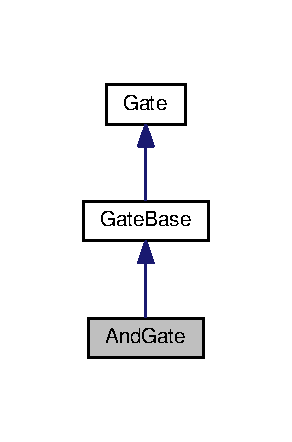
\includegraphics[width=140pt]{classAndGate__inherit__graph}
\end{center}
\end{figure}


Collaboration diagram for And\+Gate\+:
\nopagebreak
\begin{figure}[H]
\begin{center}
\leavevmode
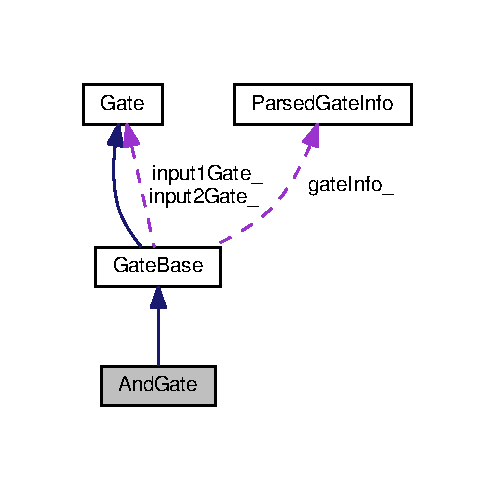
\includegraphics[width=238pt]{classAndGate__coll__graph}
\end{center}
\end{figure}
\subsection*{Public Member Functions}
\begin{DoxyCompactItemize}
\item 
{\bfseries And\+Gate} (\hyperlink{structParsedGateInfo}{Parsed\+Gate\+Info} gi)\hypertarget{classAndGate_aa235734cda4540b88abbd8351cc19431}{}\label{classAndGate_aa235734cda4540b88abbd8351cc19431}

\item 
bool {\bfseries get\+Value} () override\hypertarget{classAndGate_acc5debba56f93c67859d6acbdd1467cb}{}\label{classAndGate_acc5debba56f93c67859d6acbdd1467cb}

\end{DoxyCompactItemize}
\subsection*{Additional Inherited Members}


The documentation for this class was generated from the following file\+:\begin{DoxyCompactItemize}
\item 
Gate\+Base.\+h\end{DoxyCompactItemize}

\hypertarget{classBufGate}{}\section{Buf\+Gate Class Reference}
\label{classBufGate}\index{Buf\+Gate@{Buf\+Gate}}


Inheritance diagram for Buf\+Gate\+:
\nopagebreak
\begin{figure}[H]
\begin{center}
\leavevmode
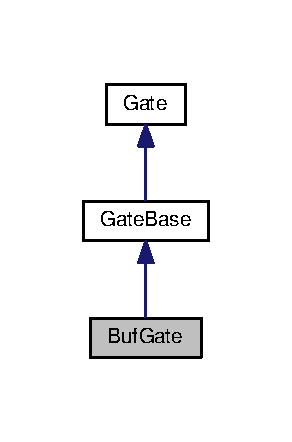
\includegraphics[width=140pt]{classBufGate__inherit__graph}
\end{center}
\end{figure}


Collaboration diagram for Buf\+Gate\+:
\nopagebreak
\begin{figure}[H]
\begin{center}
\leavevmode
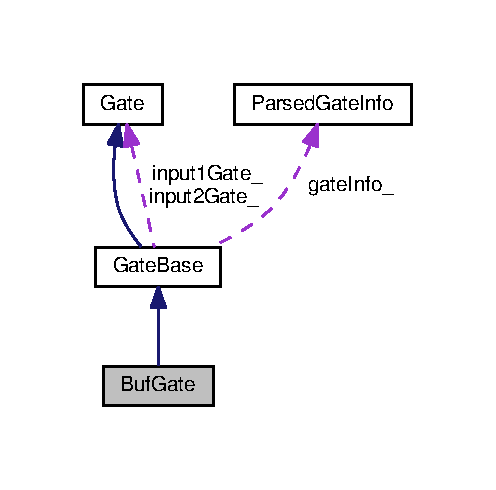
\includegraphics[width=238pt]{classBufGate__coll__graph}
\end{center}
\end{figure}
\subsection*{Public Member Functions}
\begin{DoxyCompactItemize}
\item 
{\bfseries Buf\+Gate} (\hyperlink{structParsedGateInfo}{Parsed\+Gate\+Info} gi)\hypertarget{classBufGate_a8a93571f5ce7a01add4529b5c42ee557}{}\label{classBufGate_a8a93571f5ce7a01add4529b5c42ee557}

\item 
bool {\bfseries get\+Value} () override\hypertarget{classBufGate_abb0f63b8f3a24b0d61cc142b5e8427b4}{}\label{classBufGate_abb0f63b8f3a24b0d61cc142b5e8427b4}

\end{DoxyCompactItemize}
\subsection*{Additional Inherited Members}


The documentation for this class was generated from the following file\+:\begin{DoxyCompactItemize}
\item 
Gate\+Base.\+h\end{DoxyCompactItemize}

\hypertarget{structCircuitInfo}{}\section{Circuit\+Info Struct Reference}
\label{structCircuitInfo}\index{Circuit\+Info@{Circuit\+Info}}
\subsection*{Public Attributes}
\begin{DoxyCompactItemize}
\item 
std\+::string {\bfseries circuit\+File}\hypertarget{structCircuitInfo_a4f7b8ae884ab2e7369d0707741886457}{}\label{structCircuitInfo_a4f7b8ae884ab2e7369d0707741886457}

\item 
std\+::string {\bfseries input\+Vector\+File}\hypertarget{structCircuitInfo_af4be7f92034f150f19fc25999d66c44f}{}\label{structCircuitInfo_af4be7f92034f150f19fc25999d66c44f}

\item 
std\+::string {\bfseries output\+File}\hypertarget{structCircuitInfo_a4c6698714e4faab0b11ca3df6c166f94}{}\label{structCircuitInfo_a4c6698714e4faab0b11ca3df6c166f94}

\item 
Test\+Vectors\+\_\+t {\bfseries vectors\+\_\+}\hypertarget{structCircuitInfo_a97e2f52a14b8f62282c9ce363f1f57f7}{}\label{structCircuitInfo_a97e2f52a14b8f62282c9ce363f1f57f7}

\end{DoxyCompactItemize}


The documentation for this struct was generated from the following file\+:\begin{DoxyCompactItemize}
\item 
Test\+Parser\+Info.\+h\end{DoxyCompactItemize}

\hypertarget{classCircuitParser}{}\section{Circuit\+Parser Class Reference}
\label{classCircuitParser}\index{Circuit\+Parser@{Circuit\+Parser}}
\subsection*{Public Member Functions}
\begin{DoxyCompactItemize}
\item 
{\bfseries Circuit\+Parser} (std\+::string file\+Name)\hypertarget{classCircuitParser_a0571f18af9fe330ad800f64e1dd06b13}{}\label{classCircuitParser_a0571f18af9fe330ad800f64e1dd06b13}

\item 
Parsed\+Gate\+Info\+\_\+t \& {\bfseries get\+Parsed\+Gates} ()\hypertarget{classCircuitParser_ae39eda3f3324cda0c1f50e6db8ef8600}{}\label{classCircuitParser_ae39eda3f3324cda0c1f50e6db8ef8600}

\item 
Primary\+Node\+List\+\_\+t \& {\bfseries get\+Primary\+Inputs} ()\hypertarget{classCircuitParser_a356fa2a4b05294eefab842d5cfb60153}{}\label{classCircuitParser_a356fa2a4b05294eefab842d5cfb60153}

\item 
Primary\+Node\+List\+\_\+t \& {\bfseries get\+Primary\+Outputs} ()\hypertarget{classCircuitParser_ae09c701815a66d8e217b4cb7082af0b2}{}\label{classCircuitParser_ae09c701815a66d8e217b4cb7082af0b2}

\item 
Node\+Value\+Map\+\_\+t {\bfseries get\+Input\+Node\+Values} (std\+::string \&input\+Value\+String)\hypertarget{classCircuitParser_aa2e894e75fb90c33c745c13295cf616a}{}\label{classCircuitParser_aa2e894e75fb90c33c745c13295cf616a}

\end{DoxyCompactItemize}


The documentation for this class was generated from the following files\+:\begin{DoxyCompactItemize}
\item 
Circuit\+Parser.\+h\item 
Circuit\+Parser.\+cpp\end{DoxyCompactItemize}

\hypertarget{classCircuitSimulator}{}\section{Circuit\+Simulator Class Reference}
\label{classCircuitSimulator}\index{Circuit\+Simulator@{Circuit\+Simulator}}
\subsection*{Public Member Functions}
\begin{DoxyCompactItemize}
\item 
{\bfseries Circuit\+Simulator} (const \hyperlink{classCircuitSimulator}{Circuit\+Simulator} \&)=delete\hypertarget{classCircuitSimulator_ac61805a6a803a985fc56203deda3f7a9}{}\label{classCircuitSimulator_ac61805a6a803a985fc56203deda3f7a9}

\item 
\hyperlink{classCircuitSimulator}{Circuit\+Simulator} \& {\bfseries operator=} (const \hyperlink{classCircuitSimulator}{Circuit\+Simulator} \&)=delete\hypertarget{classCircuitSimulator_a744d24f5ff23c79396930b929e54cd66}{}\label{classCircuitSimulator_a744d24f5ff23c79396930b929e54cd66}

\item 
void {\bfseries add\+Gate} (const Parsed\+Gate\+Info\+\_\+t \&gate\+Info)\hypertarget{classCircuitSimulator_a3f58ba70b4e2f16ba4c78a26359ee172}{}\label{classCircuitSimulator_a3f58ba70b4e2f16ba4c78a26359ee172}

\item 
void {\bfseries add\+Primary\+Inputs} (const Primary\+Node\+List\+\_\+t \&inputs)\hypertarget{classCircuitSimulator_a70e8ba972ffcec594f07ddd0c829469d}{}\label{classCircuitSimulator_a70e8ba972ffcec594f07ddd0c829469d}

\item 
void {\bfseries add\+Primary\+Outputs} (const Primary\+Node\+List\+\_\+t \&outputs)\hypertarget{classCircuitSimulator_aa243acfbb5baea75e5bdd4185f56020b}{}\label{classCircuitSimulator_aa243acfbb5baea75e5bdd4185f56020b}

\item 
std\+::string {\bfseries simulate} (const Node\+Value\+Map\+\_\+t \&input\+Node\+Values)\hypertarget{classCircuitSimulator_a81d8944f30b285d590809f71cfa86c3c}{}\label{classCircuitSimulator_a81d8944f30b285d590809f71cfa86c3c}

\item 
void {\bfseries reset} ()\hypertarget{classCircuitSimulator_a956e47ce8e344e707b9124803263c939}{}\label{classCircuitSimulator_a956e47ce8e344e707b9124803263c939}

\end{DoxyCompactItemize}


The documentation for this class was generated from the following files\+:\begin{DoxyCompactItemize}
\item 
Circuit\+Simulator.\+h\item 
Circuit\+Simulator.\+cpp\end{DoxyCompactItemize}

\hypertarget{classGate}{}\section{Gate Class Reference}
\label{classGate}\index{Gate@{Gate}}


Inheritance diagram for Gate\+:
\nopagebreak
\begin{figure}[H]
\begin{center}
\leavevmode
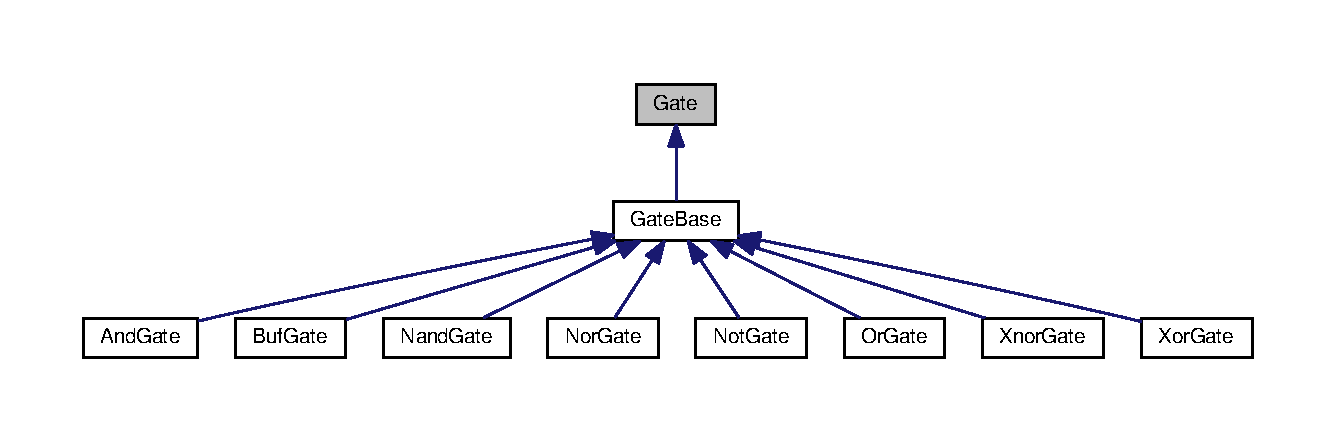
\includegraphics[width=350pt]{classGate__inherit__graph}
\end{center}
\end{figure}
\subsection*{Public Member Functions}
\begin{DoxyCompactItemize}
\item 
virtual bool {\bfseries get\+Output} ()=0\hypertarget{classGate_ac6e023a957af800cd52801cfbba0637d}{}\label{classGate_ac6e023a957af800cd52801cfbba0637d}

\item 
virtual \hyperlink{structParsedGateInfo}{Parsed\+Gate\+Info} \& {\bfseries get\+Info} ()=0\hypertarget{classGate_ac41340ef24e0e3120d48dce4e214a8f7}{}\label{classGate_ac41340ef24e0e3120d48dce4e214a8f7}

\item 
virtual void {\bfseries set\+Input1\+Gate} (\hyperlink{classGate}{Gate} $\ast$gate)=0\hypertarget{classGate_aa72a2b1c924e58600a1081710e0ec50f}{}\label{classGate_aa72a2b1c924e58600a1081710e0ec50f}

\item 
virtual void {\bfseries set\+Input2\+Gate} (\hyperlink{classGate}{Gate} $\ast$gate)=0\hypertarget{classGate_aa45e4603178df835cec2fdd9f9d12ee5}{}\label{classGate_aa45e4603178df835cec2fdd9f9d12ee5}

\item 
virtual void {\bfseries set\+Input1\+Value} (bool value)=0\hypertarget{classGate_a3d358733fa81309b5c301ab84f018f7a}{}\label{classGate_a3d358733fa81309b5c301ab84f018f7a}

\item 
virtual void {\bfseries set\+Input2\+Value} (bool value)=0\hypertarget{classGate_a0b592af9435d0089e0b68d96e49ab4c3}{}\label{classGate_a0b592af9435d0089e0b68d96e49ab4c3}

\item 
virtual void {\bfseries reset} ()=0\hypertarget{classGate_a7c5f4e00801b190c9bf984f3c3ff11c6}{}\label{classGate_a7c5f4e00801b190c9bf984f3c3ff11c6}

\end{DoxyCompactItemize}
\subsection*{Protected Member Functions}
\begin{DoxyCompactItemize}
\item 
virtual bool {\bfseries get\+Value} ()=0\hypertarget{classGate_a41c2d1a0e950f4c75d8c68f38d2b4afb}{}\label{classGate_a41c2d1a0e950f4c75d8c68f38d2b4afb}

\end{DoxyCompactItemize}


The documentation for this class was generated from the following file\+:\begin{DoxyCompactItemize}
\item 
Gate.\+h\end{DoxyCompactItemize}

\hypertarget{classGateBase}{}\section{Gate\+Base Class Reference}
\label{classGateBase}\index{Gate\+Base@{Gate\+Base}}


Inheritance diagram for Gate\+Base\+:
\nopagebreak
\begin{figure}[H]
\begin{center}
\leavevmode
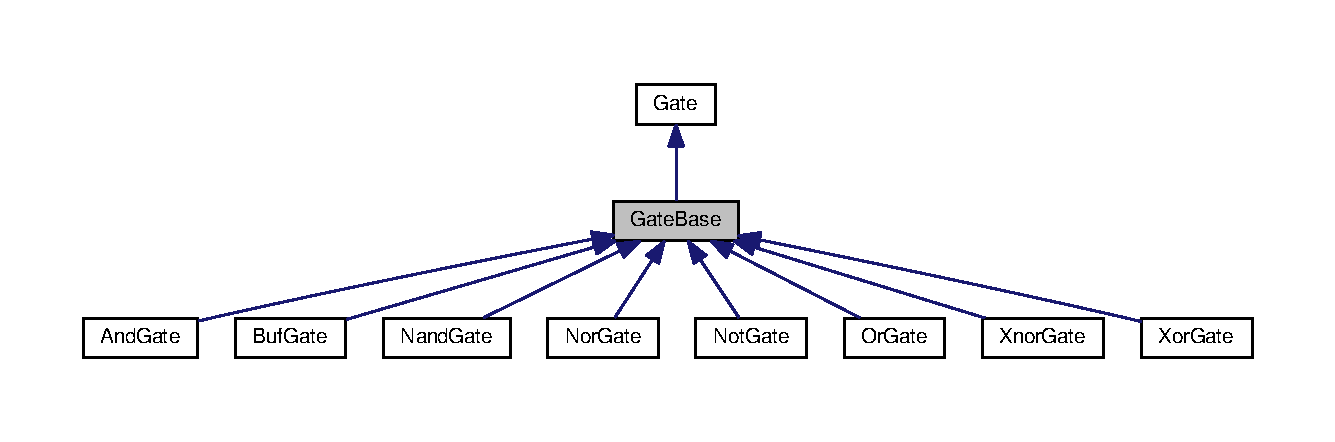
\includegraphics[width=350pt]{classGateBase__inherit__graph}
\end{center}
\end{figure}


Collaboration diagram for Gate\+Base\+:
\nopagebreak
\begin{figure}[H]
\begin{center}
\leavevmode
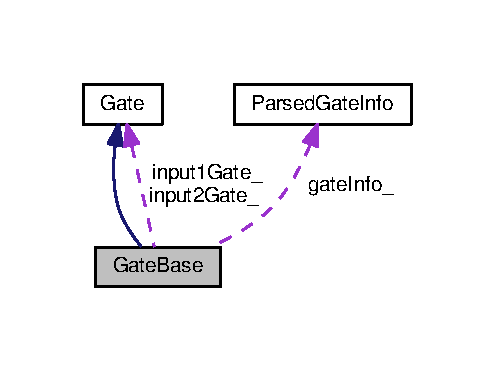
\includegraphics[width=238pt]{classGateBase__coll__graph}
\end{center}
\end{figure}
\subsection*{Public Member Functions}
\begin{DoxyCompactItemize}
\item 
{\bfseries Gate\+Base} (\hyperlink{structParsedGateInfo}{Parsed\+Gate\+Info} gi)\hypertarget{classGateBase_a5ec2f5219f1ec0f0002d264db11bf745}{}\label{classGateBase_a5ec2f5219f1ec0f0002d264db11bf745}

\item 
virtual bool {\bfseries get\+Output} () override\hypertarget{classGateBase_a8ff8ed8755b4ced0720e06701096f305}{}\label{classGateBase_a8ff8ed8755b4ced0720e06701096f305}

\item 
virtual void {\bfseries set\+Input1\+Gate} (\hyperlink{classGate}{Gate} $\ast$gate) override\hypertarget{classGateBase_a84a24d217863884116bfb22875d53e93}{}\label{classGateBase_a84a24d217863884116bfb22875d53e93}

\item 
virtual void {\bfseries set\+Input2\+Gate} (\hyperlink{classGate}{Gate} $\ast$gate) override\hypertarget{classGateBase_a3f024c6d9c20707cfc03718212008ca8}{}\label{classGateBase_a3f024c6d9c20707cfc03718212008ca8}

\item 
void {\bfseries set\+Input1\+Value} (bool value) override\hypertarget{classGateBase_aec64af0bb8332a0b6623947fa707fcee}{}\label{classGateBase_aec64af0bb8332a0b6623947fa707fcee}

\item 
void {\bfseries set\+Input2\+Value} (bool value) override\hypertarget{classGateBase_a142ad39848cf2e9ccd702c51a8cf7042}{}\label{classGateBase_a142ad39848cf2e9ccd702c51a8cf7042}

\item 
virtual \hyperlink{structParsedGateInfo}{Parsed\+Gate\+Info} \& {\bfseries get\+Info} () override\hypertarget{classGateBase_aec4a5aa00d1d2546ba690d9c9a6a6706}{}\label{classGateBase_aec4a5aa00d1d2546ba690d9c9a6a6706}

\item 
void {\bfseries reset} () override\hypertarget{classGateBase_a3d27538a156386eed5eb78f99621fd35}{}\label{classGateBase_a3d27538a156386eed5eb78f99621fd35}

\end{DoxyCompactItemize}
\subsection*{Protected Attributes}
\begin{DoxyCompactItemize}
\item 
\hyperlink{structParsedGateInfo}{Parsed\+Gate\+Info} {\bfseries gate\+Info\+\_\+}\hypertarget{classGateBase_aa8a69dba4b7d5cfae7529f1e0175d71e}{}\label{classGateBase_aa8a69dba4b7d5cfae7529f1e0175d71e}

\item 
bool {\bfseries output\+Available\+\_\+}\hypertarget{classGateBase_ae160a4ee816258d731c4f8b8803a1cc2}{}\label{classGateBase_ae160a4ee816258d731c4f8b8803a1cc2}

\item 
bool {\bfseries input1\+Value\+\_\+}\hypertarget{classGateBase_a7be516102b62c6acfa431f5d7c87b35a}{}\label{classGateBase_a7be516102b62c6acfa431f5d7c87b35a}

\item 
bool {\bfseries input2\+Value\+\_\+}\hypertarget{classGateBase_a2dcbadc2668619ca104a4239db1c4208}{}\label{classGateBase_a2dcbadc2668619ca104a4239db1c4208}

\item 
bool {\bfseries output\+Value\+\_\+}\hypertarget{classGateBase_af332cdd768672c9ecb99959196db8f59}{}\label{classGateBase_af332cdd768672c9ecb99959196db8f59}

\item 
\hyperlink{classGate}{Gate} $\ast$ {\bfseries input1\+Gate\+\_\+}\hypertarget{classGateBase_aae8c335a20c84315495da4e2f988aecf}{}\label{classGateBase_aae8c335a20c84315495da4e2f988aecf}

\item 
\hyperlink{classGate}{Gate} $\ast$ {\bfseries input2\+Gate\+\_\+}\hypertarget{classGateBase_ab3214c7cf6e29f1da6f37e08f41eccfb}{}\label{classGateBase_ab3214c7cf6e29f1da6f37e08f41eccfb}

\end{DoxyCompactItemize}
\subsection*{Additional Inherited Members}


The documentation for this class was generated from the following file\+:\begin{DoxyCompactItemize}
\item 
Gate\+Base.\+h\end{DoxyCompactItemize}

\hypertarget{classNandGate}{}\section{Nand\+Gate Class Reference}
\label{classNandGate}\index{Nand\+Gate@{Nand\+Gate}}


Inheritance diagram for Nand\+Gate\+:
\nopagebreak
\begin{figure}[H]
\begin{center}
\leavevmode
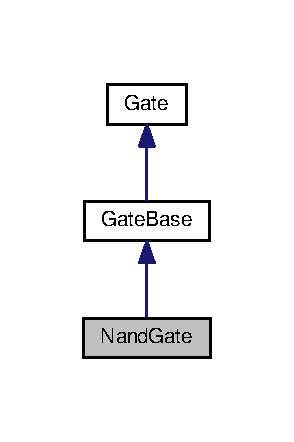
\includegraphics[width=141pt]{classNandGate__inherit__graph}
\end{center}
\end{figure}


Collaboration diagram for Nand\+Gate\+:
\nopagebreak
\begin{figure}[H]
\begin{center}
\leavevmode
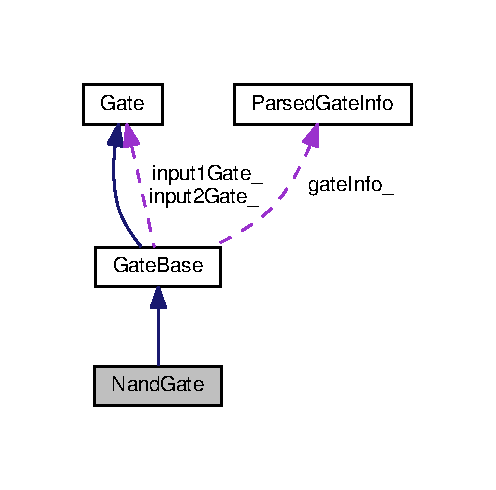
\includegraphics[width=238pt]{classNandGate__coll__graph}
\end{center}
\end{figure}
\subsection*{Public Member Functions}
\begin{DoxyCompactItemize}
\item 
{\bfseries Nand\+Gate} (\hyperlink{structParsedGateInfo}{Parsed\+Gate\+Info} gi)\hypertarget{classNandGate_a96962055c3a740014879962a83f0f90f}{}\label{classNandGate_a96962055c3a740014879962a83f0f90f}

\item 
bool {\bfseries get\+Value} () override\hypertarget{classNandGate_aaf2253a24b027624e761333fa28c3495}{}\label{classNandGate_aaf2253a24b027624e761333fa28c3495}

\end{DoxyCompactItemize}
\subsection*{Additional Inherited Members}


The documentation for this class was generated from the following file\+:\begin{DoxyCompactItemize}
\item 
Gate\+Base.\+h\end{DoxyCompactItemize}

\hypertarget{classNorGate}{}\section{Nor\+Gate Class Reference}
\label{classNorGate}\index{Nor\+Gate@{Nor\+Gate}}


Inheritance diagram for Nor\+Gate\+:
\nopagebreak
\begin{figure}[H]
\begin{center}
\leavevmode
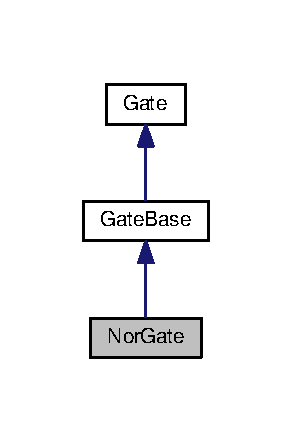
\includegraphics[width=140pt]{classNorGate__inherit__graph}
\end{center}
\end{figure}


Collaboration diagram for Nor\+Gate\+:
\nopagebreak
\begin{figure}[H]
\begin{center}
\leavevmode
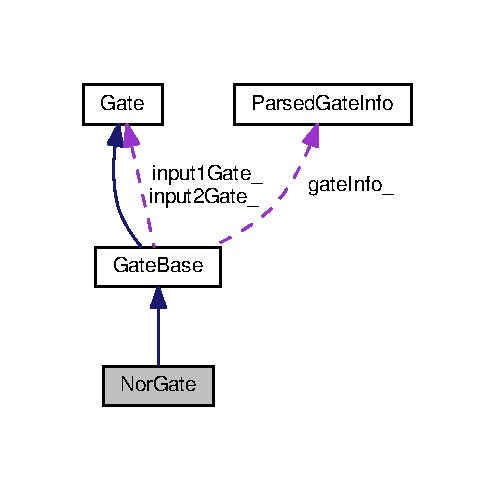
\includegraphics[width=238pt]{classNorGate__coll__graph}
\end{center}
\end{figure}
\subsection*{Public Member Functions}
\begin{DoxyCompactItemize}
\item 
{\bfseries Nor\+Gate} (\hyperlink{structParsedGateInfo}{Parsed\+Gate\+Info} gi)\hypertarget{classNorGate_a73cfc820987baef690bfb8e17881c4d6}{}\label{classNorGate_a73cfc820987baef690bfb8e17881c4d6}

\item 
bool {\bfseries get\+Value} () override\hypertarget{classNorGate_ab6f9d148efa2886aee68e0d08eedc439}{}\label{classNorGate_ab6f9d148efa2886aee68e0d08eedc439}

\end{DoxyCompactItemize}
\subsection*{Additional Inherited Members}


The documentation for this class was generated from the following file\+:\begin{DoxyCompactItemize}
\item 
Gate\+Base.\+h\end{DoxyCompactItemize}

\hypertarget{classNotGate}{}\section{Not\+Gate Class Reference}
\label{classNotGate}\index{Not\+Gate@{Not\+Gate}}


Inheritance diagram for Not\+Gate\+:
\nopagebreak
\begin{figure}[H]
\begin{center}
\leavevmode
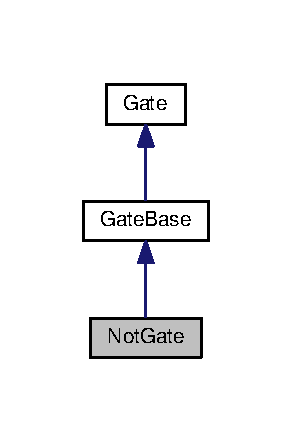
\includegraphics[width=140pt]{classNotGate__inherit__graph}
\end{center}
\end{figure}


Collaboration diagram for Not\+Gate\+:
\nopagebreak
\begin{figure}[H]
\begin{center}
\leavevmode
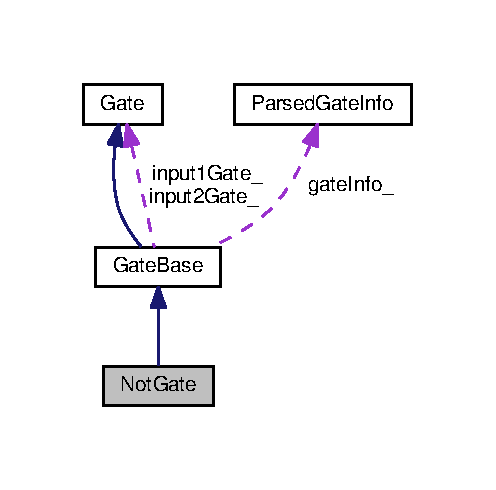
\includegraphics[width=238pt]{classNotGate__coll__graph}
\end{center}
\end{figure}
\subsection*{Public Member Functions}
\begin{DoxyCompactItemize}
\item 
{\bfseries Not\+Gate} (\hyperlink{structParsedGateInfo}{Parsed\+Gate\+Info} gi)\hypertarget{classNotGate_a7fdbc1cd0b9997d6f377ab41b97b3536}{}\label{classNotGate_a7fdbc1cd0b9997d6f377ab41b97b3536}

\item 
bool {\bfseries get\+Value} () override\hypertarget{classNotGate_a4c3c4bb46e237a8a4cab4f79175d380a}{}\label{classNotGate_a4c3c4bb46e237a8a4cab4f79175d380a}

\end{DoxyCompactItemize}
\subsection*{Additional Inherited Members}


The documentation for this class was generated from the following file\+:\begin{DoxyCompactItemize}
\item 
Gate\+Base.\+h\end{DoxyCompactItemize}

\hypertarget{classOrGate}{}\section{Or\+Gate Class Reference}
\label{classOrGate}\index{Or\+Gate@{Or\+Gate}}


Inheritance diagram for Or\+Gate\+:
\nopagebreak
\begin{figure}[H]
\begin{center}
\leavevmode
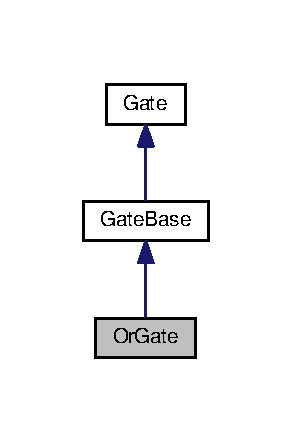
\includegraphics[width=140pt]{classOrGate__inherit__graph}
\end{center}
\end{figure}


Collaboration diagram for Or\+Gate\+:
\nopagebreak
\begin{figure}[H]
\begin{center}
\leavevmode
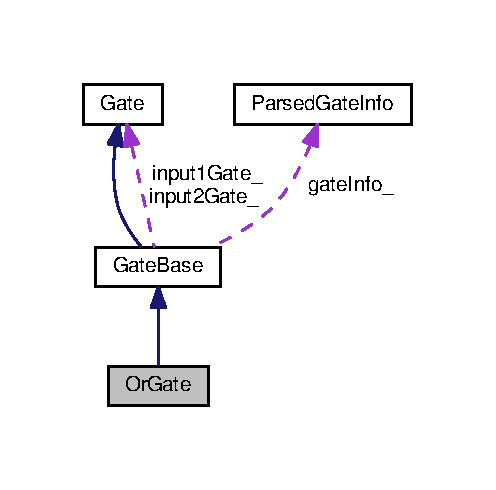
\includegraphics[width=238pt]{classOrGate__coll__graph}
\end{center}
\end{figure}
\subsection*{Public Member Functions}
\begin{DoxyCompactItemize}
\item 
{\bfseries Or\+Gate} (\hyperlink{structParsedGateInfo}{Parsed\+Gate\+Info} gi)\hypertarget{classOrGate_a10fdcd2d98fbc27ac5eec508eb7d0bad}{}\label{classOrGate_a10fdcd2d98fbc27ac5eec508eb7d0bad}

\item 
bool {\bfseries get\+Value} () override\hypertarget{classOrGate_aa012b2faf42b94a3e514402a798e2e7b}{}\label{classOrGate_aa012b2faf42b94a3e514402a798e2e7b}

\end{DoxyCompactItemize}
\subsection*{Additional Inherited Members}


The documentation for this class was generated from the following file\+:\begin{DoxyCompactItemize}
\item 
Gate\+Base.\+h\end{DoxyCompactItemize}

\hypertarget{structParsedGateInfo}{}\section{Parsed\+Gate\+Info Struct Reference}
\label{structParsedGateInfo}\index{Parsed\+Gate\+Info@{Parsed\+Gate\+Info}}
\subsection*{Public Attributes}
\begin{DoxyCompactItemize}
\item 
Gate\+Type {\bfseries gate\+Type}\hypertarget{structParsedGateInfo_a514bcd3e8895d2b4b79babee5dcd82ef}{}\label{structParsedGateInfo_a514bcd3e8895d2b4b79babee5dcd82ef}

\item 
uint32\+\_\+t {\bfseries output}\hypertarget{structParsedGateInfo_a1b1c7eb7a1273b7c212c54ee41c5f307}{}\label{structParsedGateInfo_a1b1c7eb7a1273b7c212c54ee41c5f307}

\item 
uint32\+\_\+t {\bfseries input1}\hypertarget{structParsedGateInfo_a71d56d324e35cf2c4201e0fb3f30e277}{}\label{structParsedGateInfo_a71d56d324e35cf2c4201e0fb3f30e277}

\item 
uint32\+\_\+t {\bfseries input2}\hypertarget{structParsedGateInfo_ace5809dcc3babac4f15b79ea667da859}{}\label{structParsedGateInfo_ace5809dcc3babac4f15b79ea667da859}

\end{DoxyCompactItemize}


The documentation for this struct was generated from the following file\+:\begin{DoxyCompactItemize}
\item 
Parsed\+Gate\+Info.\+h\end{DoxyCompactItemize}

\hypertarget{classTestParser}{}\section{Test\+Parser Class Reference}
\label{classTestParser}\index{Test\+Parser@{Test\+Parser}}
\subsection*{Public Member Functions}
\begin{DoxyCompactItemize}
\item 
{\bfseries Test\+Parser} (const std\+::string \&test\+File)\hypertarget{classTestParser_a29dda6e0002bf3a467599688a9ef12c1}{}\label{classTestParser_a29dda6e0002bf3a467599688a9ef12c1}

\item 
Circuits\+\_\+t \& {\bfseries get\+Circuits} ()\hypertarget{classTestParser_ab182de4b979edf9e37845514361a684f}{}\label{classTestParser_ab182de4b979edf9e37845514361a684f}

\item 
void {\bfseries print\+Summary} ()\hypertarget{classTestParser_ac781d3262fa87c7c36f667d01e014c34}{}\label{classTestParser_ac781d3262fa87c7c36f667d01e014c34}

\end{DoxyCompactItemize}


The documentation for this class was generated from the following files\+:\begin{DoxyCompactItemize}
\item 
Test\+Parser.\+h\item 
Test\+Parser.\+cpp\end{DoxyCompactItemize}

\hypertarget{structTestVector}{}\section{Test\+Vector Struct Reference}
\label{structTestVector}\index{Test\+Vector@{Test\+Vector}}
\subsection*{Public Member Functions}
\begin{DoxyCompactItemize}
\item 
{\bfseries Test\+Vector} (std\+::string input, std\+::string expected\+Output=\char`\"{}\char`\"{})\hypertarget{structTestVector_a060e66ed253d04a71d65a4257f74eb2d}{}\label{structTestVector_a060e66ed253d04a71d65a4257f74eb2d}

\end{DoxyCompactItemize}
\subsection*{Public Attributes}
\begin{DoxyCompactItemize}
\item 
std\+::string {\bfseries input}\hypertarget{structTestVector_ace4526fda14e70cfe0cff2459cdb0cbc}{}\label{structTestVector_ace4526fda14e70cfe0cff2459cdb0cbc}

\item 
std\+::string {\bfseries expected\+Output}\hypertarget{structTestVector_a28f486ddc9f19a60408f4ac34c482011}{}\label{structTestVector_a28f486ddc9f19a60408f4ac34c482011}

\item 
std\+::string {\bfseries output}\hypertarget{structTestVector_aabadde25dd47628deb43051d0db31324}{}\label{structTestVector_aabadde25dd47628deb43051d0db31324}

\end{DoxyCompactItemize}


The documentation for this struct was generated from the following file\+:\begin{DoxyCompactItemize}
\item 
Test\+Parser\+Info.\+h\end{DoxyCompactItemize}

\hypertarget{classXnorGate}{}\section{Xnor\+Gate Class Reference}
\label{classXnorGate}\index{Xnor\+Gate@{Xnor\+Gate}}


Inheritance diagram for Xnor\+Gate\+:
\nopagebreak
\begin{figure}[H]
\begin{center}
\leavevmode
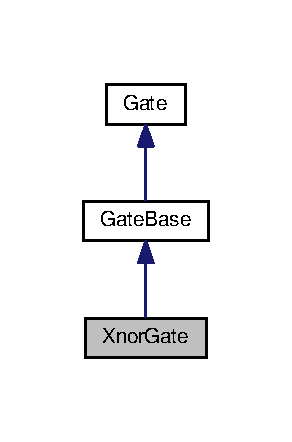
\includegraphics[width=140pt]{classXnorGate__inherit__graph}
\end{center}
\end{figure}


Collaboration diagram for Xnor\+Gate\+:
\nopagebreak
\begin{figure}[H]
\begin{center}
\leavevmode
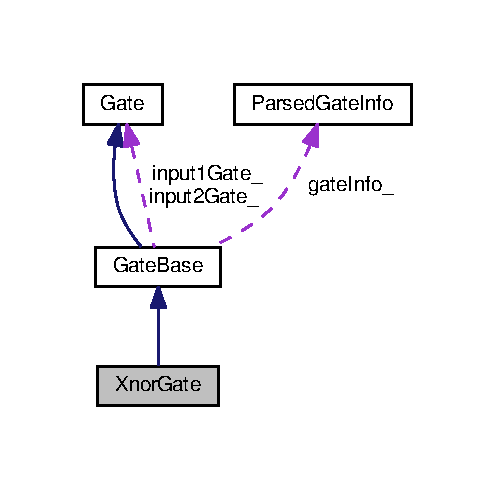
\includegraphics[width=238pt]{classXnorGate__coll__graph}
\end{center}
\end{figure}
\subsection*{Public Member Functions}
\begin{DoxyCompactItemize}
\item 
{\bfseries Xnor\+Gate} (\hyperlink{structParsedGateInfo}{Parsed\+Gate\+Info} gi)\hypertarget{classXnorGate_a8fdae6109d50e3ede521261d100dd0f1}{}\label{classXnorGate_a8fdae6109d50e3ede521261d100dd0f1}

\item 
bool {\bfseries get\+Value} () override\hypertarget{classXnorGate_aaf83cf68772ffbc963853acd60571f06}{}\label{classXnorGate_aaf83cf68772ffbc963853acd60571f06}

\end{DoxyCompactItemize}
\subsection*{Additional Inherited Members}


The documentation for this class was generated from the following file\+:\begin{DoxyCompactItemize}
\item 
Gate\+Base.\+h\end{DoxyCompactItemize}

\hypertarget{classXorGate}{}\section{Xor\+Gate Class Reference}
\label{classXorGate}\index{Xor\+Gate@{Xor\+Gate}}


Inheritance diagram for Xor\+Gate\+:
\nopagebreak
\begin{figure}[H]
\begin{center}
\leavevmode
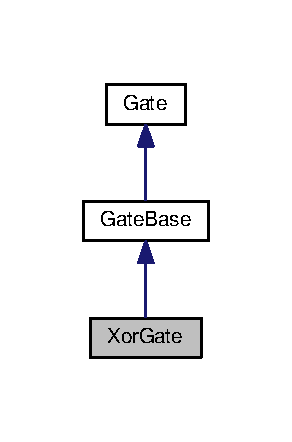
\includegraphics[width=140pt]{classXorGate__inherit__graph}
\end{center}
\end{figure}


Collaboration diagram for Xor\+Gate\+:
\nopagebreak
\begin{figure}[H]
\begin{center}
\leavevmode
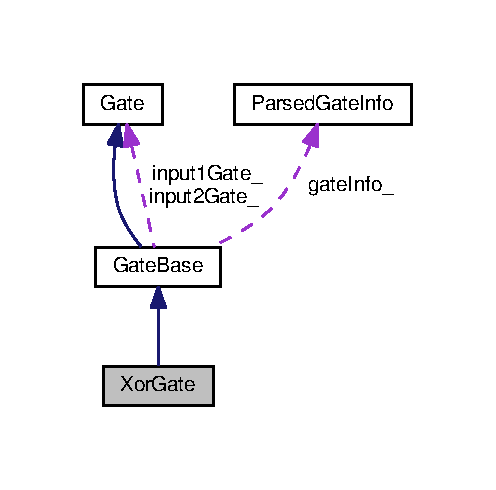
\includegraphics[width=238pt]{classXorGate__coll__graph}
\end{center}
\end{figure}
\subsection*{Public Member Functions}
\begin{DoxyCompactItemize}
\item 
{\bfseries Xor\+Gate} (\hyperlink{structParsedGateInfo}{Parsed\+Gate\+Info} gi)\hypertarget{classXorGate_aedcc41a85beb20e76d0c63233cc4dec7}{}\label{classXorGate_aedcc41a85beb20e76d0c63233cc4dec7}

\item 
bool {\bfseries get\+Value} () override\hypertarget{classXorGate_a2650b38740d17322fec0af68b7e9a10e}{}\label{classXorGate_a2650b38740d17322fec0af68b7e9a10e}

\end{DoxyCompactItemize}
\subsection*{Additional Inherited Members}


The documentation for this class was generated from the following file\+:\begin{DoxyCompactItemize}
\item 
Gate\+Base.\+h\end{DoxyCompactItemize}

%--- End generated contents ---

% Index
\backmatter
\newpage
\phantomsection
\clearemptydoublepage
\addcontentsline{toc}{chapter}{Index}
\printindex

\end{document}
